%%%%%%%%%%%%%%%%%%%%%%%%%%%%%%%%%%%%%%%%%%%%%%%%%%%%%%%%%%%%%%%%%%%%%%%
\documentclass{beamer}
\mode<presentation>
\usepackage{beamerthemesplit}
%\usepackage{verbatim}
\usepackage{hyperref}
\usepackage{setspace}
\usepackage{xcolor}
\usepackage{listings}
\usepackage[normalem]{ulem}
\usetheme{Madrid}
\usecolortheme{default}
\setbeamerfont*{frametitle}{size=\normalsize}
\setbeamertemplate{navigation symbols}{}
%%%%%%%%%%%%%%%%%%%%%%%%%%%%%%%%%%%%%%%%%%%%%%%%%%%%%%%%%%%%%%%%%%%%%%%


%%%%%%%%%%%%%%%%%%%%%%%%%%%%%%%%%%%%%%%%%%%%%%%%%%%%%%%%%%%%%%%%%%%%%%%
\title[Prog4Chem]{Spring 2025: Programming for chemistry}
\subtitle{(in Python!)}
\author[Davide Ceresoli]{Davide Ceresoli (davide.ceresoli@cnr.it)}
\date{\today}
\institute[CNR-SCITEC]{Instituto di Scienze e Tecnologie Chimiche ``G. Natta'' (CNR-SCITEC)}
\pgfdeclareimage[height=.7cm]{university-logo}{gg_scitec_logo_2_colore.png}
\logo{\pgfuseimage{university-logo}}

%%%%%%%%%%%%%%%%%%%%%%%%%%%%%%%%%%%%%%%%%%%%%%%%%%%%%%%%%%%%%%%%%%%%%%%
\begin{document}
%%%%%%%%%%%%%%%%%%%%%%%%%%%%%%%%%%%%%%%%%%%%%%%%%%%%%%%%%%%%%%%%%%%%%%%
\begin{frame}
\titlepage
\end{frame}

\begin{frame}{Outline}
\tableofcontents
\end{frame}



%%%%%%%%%%%%%%%%%%%%%%%%%%%%%%%%%%%%%%%%%%%%%%%%%%%%%%%%%%%%%%%%%%%%%%%
\section{Course logistics}
%%%%%%%%%%%%%%%%%%%%%%%%%%%%%%%%%%%%%%%%%%%%%%%%%%%%%%%%%%%%%%%%%%%%%%%
\begin{frame}[fragile]
  \frametitle{Introduction}
  \begin{itemize}
  \item Dr Davide Ceresoli, Senior Researcher at CNR-SCITEC
  \item office phone: 02-503-14276
  \item email: davide.ceresoli@cnr.it 
  \item background: \emph{laurea} in Materials Science, PhD in Physics
  \item activity: ab-initio DFT calculations, molecular dynamics, high-prssure, thermoelectrics, code development (Quantum-Espresso)  
  \end{itemize}
\end{frame}

\begin{frame}[fragile]
  \frametitle{Course organization}
  \begin{itemize}
  \item 6 CFU, 48 hours (24 lectures two hours each)
  \item lectures (settore didattico via Celoria):
        \begin{itemize}
        \item tuesdays 08:30-10:30, room ???
        \item fridays 08:30-10:30, room ???
        \end{itemize}
  \item course website: \url{https://dceresoli.github.io/2025-Programming}
  \end{itemize}
  \begin{center}
  
\includegraphics[width=4cm]{QR.png}
  \end{center}
\end{frame}

\begin{frame}[fragile]
  \frametitle{Course objectives}
  \begin{itemize}
  \item No previous knowledge of programming is assumed!\pause
  \item By the end of the course, you will:\pause
        \begin{itemize}
        \item Understand fundamental concepts of programming imperative languages
        \item Design algorithms to solve simple problems
        \item Learn the Python programming language
        \item Solve some chemistry-related problems
        \item Have fun programming, maybe a computer game...
        \end{itemize}
  \end{itemize}
\end{frame}

\begin{frame}[fragile]
  \frametitle{Textbook and reference material}
  \begin{itemize}
  \item There are plenty of online free Python books, tutorials and resources
  \item P. Wentworth \emph{et al.}, \emph{How to Think Like a Computer Scientist in Python 3}, 
        available free at: \url{https://openbookproject.net/thinkcs/python/english3e/}
  \item The official Python 3 documentation: \url{https://docs.python.org/3/}
  \end{itemize}
\end{frame}

\begin{frame}[fragile]
  \frametitle{Programming tools: Python + Jupyter}
  \begin{itemize}
  \item We'll use the interactive Jupyter notebook most of the time. Here are the tools you need to install:\pause
  \item Windows: Anaconda \textsl{\small{(too much user friendly!)}}\pause
  \item Windows: WSL with Debian/Ubuntu\\
       \verb|sudo apt install python3 jupyter numpy scipy matplotlib|
  \item \textbf{Linux} and \textbf{VSCode} \textsl{\small{(the only Microsoft-product that works!)}}\pause
  \item Mac OS: I have no idea!\pause
  \item In the cloud: Google Colab \url{https://colab.research.google.com/}
  \end{itemize}
\end{frame}
 
\begin{frame}[fragile]
  \frametitle{Policies and grading}
  \begin{itemize}
  \item Lectures: can be interactive, with questions and  interactive problem solving\pause
  \item Attendance is recommended\pause
  \item \textbf{You are not allowed to use AI assistants such as: ChatGPT, Claude, Gemini!}\pause
  \item There will be two ``free programming practice'' days to catch up, exercise, propose problems\pause
  \item Final exam: oral, couple of general questions, coding 3--4 notebook cells 
  \end{itemize}
\end{frame}

\begin{frame}
   \frametitle{}
   \begin{center}
   Questions?
   \end{center}
\end{frame}

%%%%%%%%%%%%%%%%%%%%%%%%%%%%%%%%%%%%%%%%%%%%%%%%%%%%%%%%%%%%%%%%%%%%%%%
\section{The way to program}
%%%%%%%%%%%%%%%%%%%%%%%%%%%%%%%%%%%%%%%%%%%%%%%%%%%%%%%%%%%%%%%%%%%%%%%
\begin{frame}[fragile]
  \frametitle{Modern computer architecture}
  \begin{center}
  
\includegraphics[width=0.6\textwidth]{computer_comic.png}
  \end{center}
  \begin{block}{Take-home message}
  Computer don't solve problems (yet), people do!
  \end{block}
\end{frame}

\begin{frame}[fragile]
  \frametitle{Modern computer architecture}
  \begin{center}
  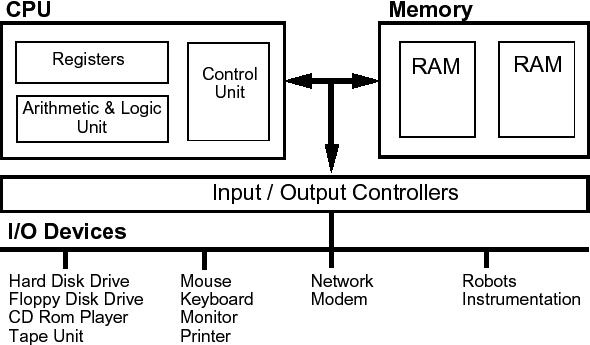
\includegraphics[width=0.8\textwidth]{computer_architecture.png}
  \end{center}
\end{frame}

\begin{frame}[fragile]
  \frametitle{The CPU}
  \begin{center}
  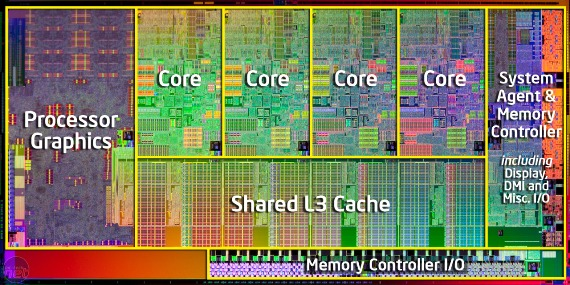
\includegraphics[width=0.5\textwidth]{insideintel.jpg}
  \end{center}
  \begin{itemize}
  \item The CPU reads the both code and data from RAM
  \item The code is executed one instruction at the time, data is
        moved to/from memory
  \item Conditionally, the CPU jumps to a different location in the code\pause
  \item The operating system (OS) takes care of:
        \begin{itemize} 
        \item scheduling execution of $N$ processes on $m$ CPU cores
        \item move data to/from disk, network and RAM
        \item interact with the hardware and with the user
        \end{itemize}
  \end{itemize} 
\end{frame}

\begin{frame}[fragile]
  \frametitle{Low-level language}
  \begin{block}{}
  The CPU understands only low-level \emph{Assembly} instructions
  \end{block}
  \begin{columns}
  \begin{column}[T]{0.4\textwidth}
  \begin{itemize}
  \item This are very simple instructions such as:
        \begin{itemize} 
        \item move bytes from RAM to CPU registers and back
        \item do arithmetic operations on CPU registers
        \item advance to the next instruction, or jump to an other
              location
        \item each CPU has a different set of instructions!
        \end{itemize}
  \end{itemize}
  \end{column}
  \begin{column}[T]{0.6\textwidth}
  \lstset{language=C++,basicstyle=\tiny\ttfamily}
  \begin{lstlisting}
Disassembly of section .text:

0000000000000000 <distance>:
   0:	55                   	push   %rbp
   1:	48 89 e5             	mov    %rsp,%rbp
   4:	48 83 ec 20          	sub    $0x20,%rsp
   8:	f2 0f 11 45 f8       	movsd  %xmm0,-0x8(%rbp)
   d:	f2 0f 11 4d f0       	movsd  %xmm1,-0x10(%rbp)
  12:	f2 0f 11 55 e8       	movsd  %xmm2,-0x18(%rbp)
  17:	f2 0f 10 45 f8       	movsd  -0x8(%rbp),%xmm0
  1c:	66 0f 28 c8          	movapd %xmm0,%xmm1
  20:	f2 0f 59 4d f8       	mulsd  -0x8(%rbp),%xmm1
  25:	f2 0f 10 45 f0       	movsd  -0x10(%rbp),%xmm0
  2a:	f2 0f 59 45 f0       	mulsd  -0x10(%rbp),%xmm0
  2f:	f2 0f 58 c8          	addsd  %xmm0,%xmm1
  33:	f2 0f 10 45 e8       	movsd  -0x18(%rbp),%xmm0
  38:	f2 0f 59 45 e8       	mulsd  -0x18(%rbp),%xmm0
  3d:	f2 0f 58 c1          	addsd  %xmm1,%xmm0
  41:	e8 00 00 00 00       	callq  46 <distance+0x46>
  46:	f2 0f 11 45 e0       	movsd  %xmm0,-0x20(%rbp)
  4b:	48 8b 45 e0          	mov    -0x20(%rbp),%rax
  4f:	48 89 45 e0          	mov    %rax,-0x20(%rbp)
  53:	f2 0f 10 45 e0       	movsd  -0x20(%rbp),%xmm0
  58:	c9                   	leaveq 
  59:	c3                   	retq   
  \end{lstlisting}
  \end{column}
  \end{columns}
\end{frame}

\begin{frame}[fragile]
  \frametitle{High-level languages}
  \begin{block}{}
  For us, it is easier to program in higher-level languages
  \end{block}
  \vspace{1cm}
  The previous block of bytes and assembly instructions, is
  equivalent to:
  \lstset{language=C++,basicstyle=\small\ttfamily,keywordstyle=\color{blue},
  stringstyle=\color{green},numberstyle=\color{red}}
  \begin{lstlisting}
#include <math.h>

double distance(double x, double y, double z)
{
   return sqrt(x*x + y*y + z*z);
}
  \end{lstlisting}\pause
  \begin{block}{This code runs on almost every CPU}
  This is why we need to learn programming languages!
  \end{block}
\end{frame}

\begin{frame}[fragile]
  \frametitle{From source code to CPU instructions}
  \begin{block}{Compiled languages}
  \begin{itemize}
  \item Source code is analyzed entirely and checked for errors\pause
  \item Then, the source code is \emph{compiled} (aka translated) into assembly instructions\pause
  \item Possibility to perform deep code optimizations\pause
  \item Finally, multiple code units are \emph{linked} together and with
        \emph{libraries} of functions\pause
  \item The results is the \emph{executable}, that can be run by the operating system
        \emph{at the maximum performance}\pause
  \item Compiled languages: C, C++, Fortran, Pascal, Go, Rust, ...
  \end{itemize}
  \end{block}
\end{frame}

\begin{frame}[fragile]
  \frametitle{From source code to CPU instructions}
  \begin{block}{Interpreted languages}
  \begin{itemize}
  \item Source code is processed line-by-line and checked for errors\pause
  \item The interpreter \emph{runs} the source code, also interactively\pause
  \item Possibility to debug and inspect the code while writing\pause
  \item Usually very easy and fun to program with\pause
  \item Difficult to optimize, performance much lower than compiled languages\pause
  \item Interpreted languages: Python, Basic, Forth, Javascript, PHP, Lisp, Octave, ...
  \end{itemize}
  \end{block}
\end{frame}

\begin{frame}[fragile]
  \frametitle{From source code to CPU instructions}
  \begin{block}{In the middle: just-in-time compiled languages}
  \begin{itemize}
  \item Source code is processed line-by-line and checked for errors,
        also interactively\pause
  \item The code is compiled \emph{on-the-fly} to CPU instructions\pause
  \item Performance is between compiled and interpreted languages\pause
  \item Price to pay is longer startup time and need of support run-time
        libraries\pause
  \item JIT languages: Java, Javascript, Julia, Wasm, ...
  \end{itemize}
  \end{block}
\end{frame}

\begin{frame}[fragile]
  \frametitle{From source code to CPU instructions}
  \begin{block}{In the middle: just-in-time compiled languages}
  \begin{itemize}
  \item Source code is processed line-by-line and checked for errors,
        also interactively\pause
  \item The code is compiled \emph{on-the-fly} to CPU instructions\pause
  \item Performance is between compiled and interpreted languages\pause
  \item Price to pay is longer startup time and need of support run-time
        libraries\pause
  \item JIT languages: Java, Javascript, Julia, Wasm, ...
  \end{itemize}
  \end{block}
\end{frame}

\begin{frame}[fragile]
  \frametitle{Programming language popularity}
  \begin{center}
  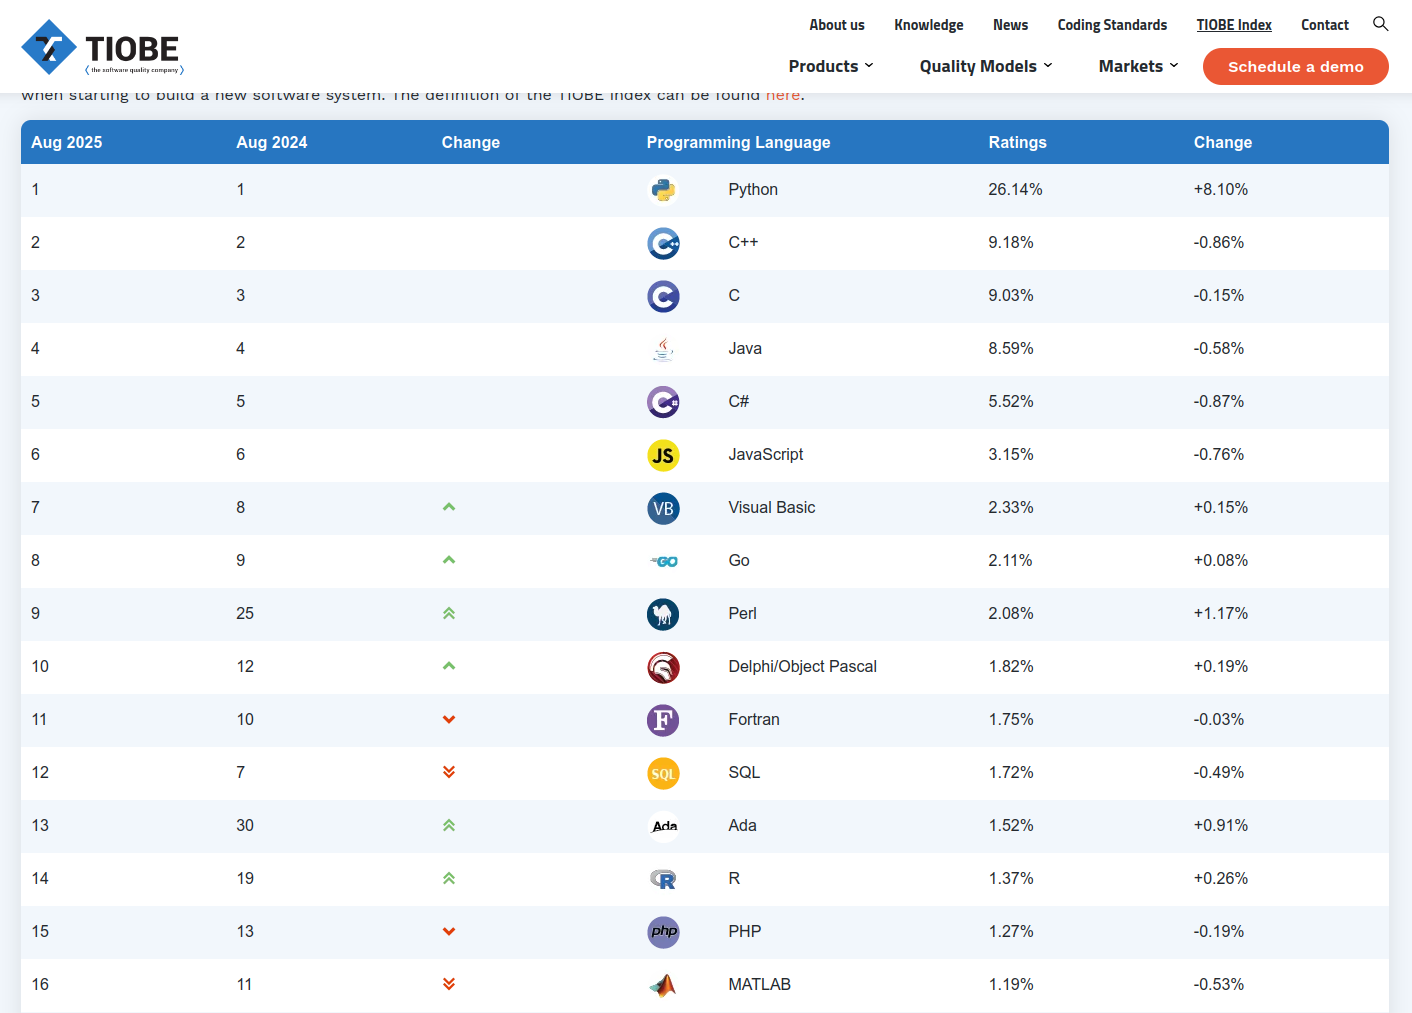
\includegraphics[width=0.95\textwidth]{TIOBE-2025.png}
  \end{center}
\end{frame}

\begin{frame}[fragile]
  \frametitle{Why Python?}
  \begin{block}{Python is slow!}
  \begin{itemize}
  \item Can be 100x times slower than C/C++/Fortran
  \end{itemize}
  \end{block}\pause
  \begin{block}{Python is fast!}
  \begin{itemize}
  \item If you use C/C++/Fortran libraries
  \end{itemize}
  \end{block}\pause
  \begin{alertblock}{}
  \centering Julia is emerging as a fast and powerful language for scientific programming
  \end{alertblock}
\end{frame}


%%%%%%%%%%%%%%%%%%%%%%%%%%%%%%%%%%%%%%%%%%%%%%%%%%%%%%%%%%%%%%%%%%%%%%%
\section{The Python programming language}
%%%%%%%%%%%%%%%%%%%%%%%%%%%%%%%%%%%%%%%%%%%%%%%%%%%%%%%%%%%%%%%%%%%%%%%
\begin{frame}[fragile]
  \frametitle{The Python programming language}
  \begin{itemize}
  \item Conceived by Guido van Rossum in the '90s (Python 1)
  \item Python 2 was popular until few years ago, not used anymore
  \item We'll be using at least Python 3.11 (shipped with Linux Debian 12)
  \item Python 2 and Python 3 are incompatible, the code must be converted
  \item \emph{I will point out major differences between Python and other programming languages}
  \end{itemize}
\end{frame}

\begin{frame}[fragile]
  \frametitle{How does Python look like?}
  \lstset{language=Python,basicstyle=\tiny\ttfamily,keywordstyle=\color{blue}, stringstyle=\color{green},numberstyle=\color{red}]}
  \begin{lstlisting}
#!/usr/bin/env python
# Anderson model in 2d

import numpy as np
import numpy.random as random
import scipy.sparse as sparse
from scipy.sparse.linalg import eigs, eigsh
import matplotlib.pyplot as plt

# number of sites
Nx, Ny = 100, 100

# hopping and randomness
t = 1.0
r = 0.1

# setup hamiltonian
N = Nx*Ny
H = sparse.lil_matrix((N,N))
H.setdiag(r*random.randn(N))

for ix in range(Nx):
    for iy in range(Ny):
        i = ix*Ny + iy
        H[i,(i+1) % N] = t
        H[i,i-1] = t
        H[i,(i+Ny) % N] = t
        H[i,i-Ny] = t
...
  \end{lstlisting}
\end{frame}

\begin{frame}[fragile]
  \frametitle{The Python language}
  \begin{block}{Pros}
    \begin{itemize}
    \item Imperative, structured (make use of ``functions''), modules
    \item Plenty of existing libraries and modules
    \item More than one way to write an algorithm
    \item {\color{green} Easy to learn!}
    \end{itemize}
  \end{block}\pause
  \begin{block}{Cons}
    \begin{itemize}
    \item Easy to mess up with data types
    \item Not CPU and memory efficient
    \item {\color{red} Easy to make mistakes!}
    \end{itemize}
  \end{block}
\end{frame}

\begin{frame}[fragile]
  \frametitle{Our first Python program (Linux shell}
  \begin{center}
  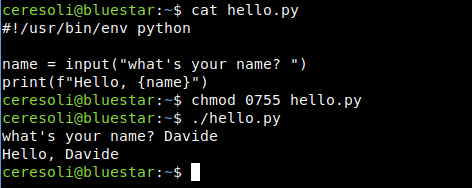
\includegraphics[width=0.8\textwidth]{hello_cli.png}
  \end{center}
  \begin{center}
  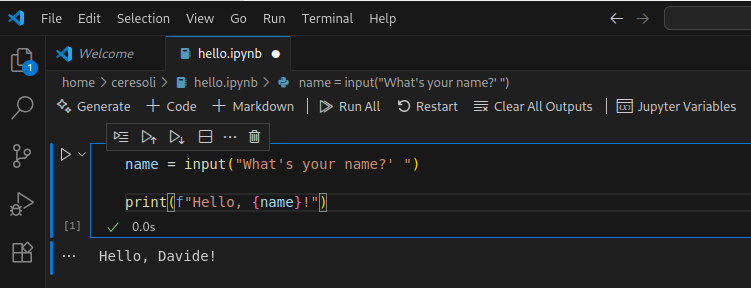
\includegraphics[width=0.8\textwidth]{hello_vscode.png}
  \end{center}
\end{frame}

\begin{frame}[fragile]
  \frametitle{Our first Python program (VScode}
  \begin{center}
  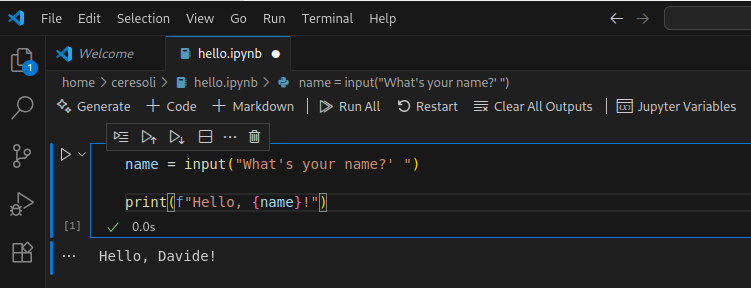
\includegraphics[width=0.8\textwidth]{hello_vscode.png}
  \end{center}
\end{frame}


\begin{frame}[fragile]
  \frametitle{Our first Python program (Jupyter}
  \begin{center}
  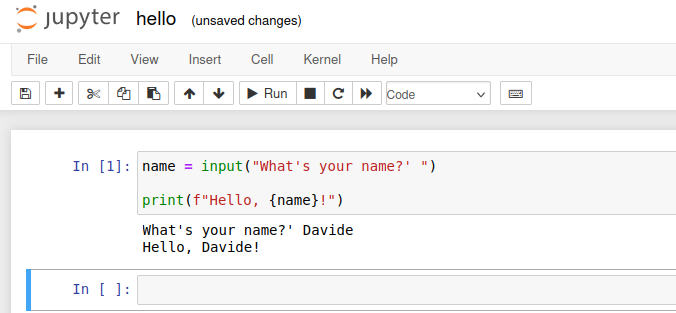
\includegraphics[width=0.8\textwidth]{hello_jupyter.png}
  \end{center}
\end{frame}


\begin{frame}[fragile]
  \frametitle{Let's try it}
  \begin{center}
  \Huge{Time to install and setup Python!}
  \end{center}
  \vspace{2cm}
  \begin{center}
  Next step: download lecture \#1 notebook from \url{https://github.com/dceresoli/2025-Programming}.
  \end{center}
\end{frame}



%%%%%%%%%%%%%%%%%%%%%%%%%%%%%%%%%%%%%%%%%%%%%%%%%%%%%%%%%%%%%%%%%%%%%%%
\section{Recap}
%%%%%%%%%%%%%%%%%%%%%%%%%%%%%%%%%%%%%%%%%%%%%%%%%%%%%%%%%%%%%%%%%%%%%%%
\begin{frame}[fragile]
  \frametitle{Recap}
  \begin{itemize}
  \item Low-level vs high-level languages\pause
  \item Compilers vs interpreters\pause
  \item The first program in Python\pause
  \item Interactive coding with Jupyter notebooks\pause
  \end{itemize}
  \begin{block}{}
  \begin{center}Questions?\end{center}
  \end{block}
\end{frame}


%%%%%%%%%%%%%%%%%%%%%%%%%%%%%%%%%%%%%%%%%%%%%%%%%%%%%%%%%%%%%%%%%%%%%%%
\end{document}
%%%%%%%%%%%%%%%%%%%%%%%%%%%%%%%%%%%%%%%%%%%%%%%%%%%%%%%%%%%%%%%%%%%%%%%


